%!TEX root=../../main.tex

%_______________
\section{Exercises}



%_______________
\subsection{Variability in estimates}

% 1 oi_biostat, blue_eggs

\eoce{\qt{Egg coloration\label{blue_eggs}} The evolutionary role of variation in bird egg coloration remains mysterious to biologists. One hypothesis suggests that egg color may play a role in sexual selection. For example, perhaps healthier females are able to deposit more blue-green pigment into eggshells instead of using it themselves as an antioxidant. Researchers measured the blue-green chroma (BGC) of 70 different collared flycatcher nests in an area of the Czech Republic.
	
	\begin{minipage}[c]{0.75\textwidth}
		\begin{center}
			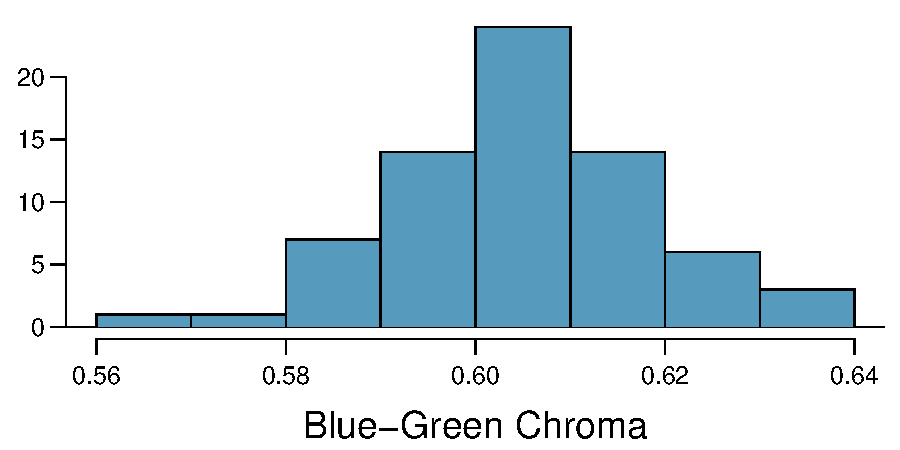
\includegraphics[width=\textwidth]{ch_inference_foundations_oi_biostat/figures/eoce/blue_eggs/blue_eggs_hist.pdf}
		\end{center}
	\end{minipage}
	\begin{minipage}[c]{0.22\textwidth}
		\begin{center}
			\begin{tabular}{l|r l}
				Min     & 0.5675 \\
				Q1      & 0.5977 \\
				Median  & 0.6046 \\
				Mean    & 0.6052 \\
				SD      & 0.0131 \\
				Q3      & 0.6126 \\
				Max     & 0.6355 \\
			\end{tabular}
		\end{center}
	\end{minipage}	
	\begin{parts}
		\item What is the point estimate for the average BGC of nests?
		\item What is the point estimate for the standard deviation of the BGC of eggs across nests?
		\item Would a nest with average BGC of 0.63 be considered unusually high? Explain your reasoning.
		\item Compute the standard error of the sample mean using the summary statistics.
	\end{parts}
}{}

\textD{\newpage}

% 2 EVEN (OI 4.4) edited

\eoce{\qt{Heights of adults\label{adult_heights}} Researchers studying anthropometry 
collected body girth measurements and skeletal diameter measurements, as well as 
age, weight, height and gender, for 507 physically active individuals. The 
histogram below shows the sample distribution of heights in centimeters. 
\footfullcite{Heinz:2003} \\
\begin{minipage}[c]{0.75\textwidth}
\begin{center}
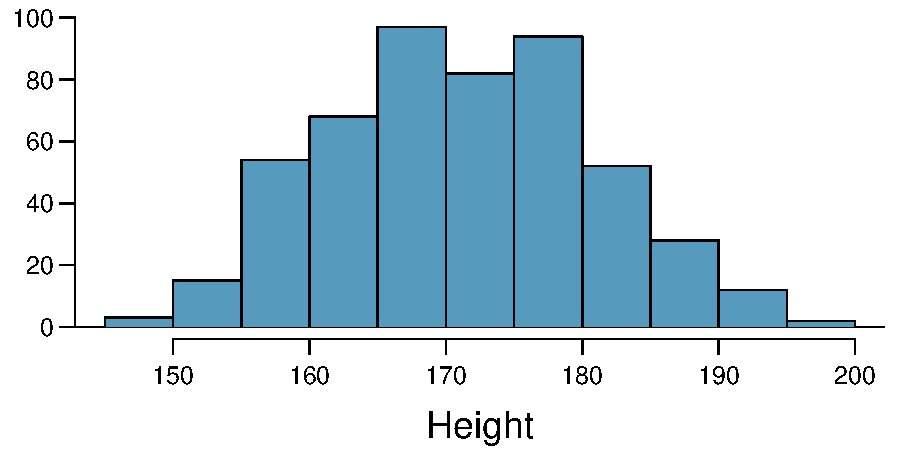
\includegraphics[width=\textwidth]{ch_inference_foundations_oi_biostat/figures/eoce/adult_heights/adult_heights_hist.pdf}
\end{center}
\end{minipage}
\begin{minipage}[c]{0.23\textwidth}
\begin{center}
\begin{tabular}{l|r l}
Min     & 147.2 \\
Q1      & 163.8 \\
Median  & 170.3 \\
Mean    & 171.1 \\
SD      &  9.4 \\
Q3      & 177.8 \\
Max     & 198.1 \\
\end{tabular}
\end{center}
\end{minipage}
\begin{parts}
\item What is the point estimate for the average height of active individuals? 
\item What is the point estimate for the standard deviation of the heights of 
active individuals? What about the IQR?
\item Is a person who is 1m 80cm (180 cm) tall considered unusually tall? And is 
a person who is 1m 55cm (155cm) considered unusually short? Explain your 
reasoning.
\item The researchers take another random sample of physically active 
individuals. Would you expect the mean and the standard deviation of this new 
sample to be the ones given above? Explain your reasoning.
\item The sample means obtained are point estimates for the mean height of all 
active individuals, if the sample of individuals is equivalent to a simple 
random sample. What measure is used to quantify the variability of such an 
estimate? Compute this quantity using the data from the original sample under the condition that the data are a simple random sample. 
\end{parts}
}{}


% 3 ODD (OI3, 4.5)

\eoce{\qt{Hen eggs\label{hen_eggs}} The distribution of the number of eggs laid 
by a certain species of hen during their breeding period is on average, 35 eggs,  
with a standard deviation of 18.2. Suppose a group of researchers 
randomly samples 45 hens of this species, counts the number of eggs laid 
during their breeding period, and records the sample mean. They repeat 
this 1,000 times, and build a distribution of sample means.
 
\begin{parts}
\item What is this distribution called? 
\item Would you expect the shape of this distribution to be symmetric, right 
skewed, or left skewed? Explain your reasoning.
\item Calculate the variability of this distribution and state the appropriate 
term used to refer to this value.
\item Suppose the researchers' budget is reduced and they are only able to 
collect random samples of 10 hens. The sample mean of the number of eggs is 
recorded, and we repeat this 1,000 times, and build a new distribution of sample 
means. How will the variability of this new distribution compare to the 
variability of the original distribution?
\end{parts}
}{}


\textD{\newpage}


%_______________
\subsection{Confidence intervals}

% 4 EVEN (OI3, 4.12) edited

\eoce{\qt{Mental health, Part I\label{mental_health}} The 2010 General Social Survey asked the question: ``For how many days during the past 30 days was your 
	mental health, which includes stress, depression, and problems with emotions, 
	not good?" Based on responses from 1,151 US residents, the survey reported a 95\%
	confidence interval of 3.40 to 4.24 days in 2010.
	\begin{parts}
		\item Interpret this interval in context of the data.
		\item What does ``95\% confident" mean? Explain in the context of the application.
		\item If a new survey were to be done with 500 Americans, would the standard 
		error of the estimate be larger, smaller, or about the same? Assume the standard 
		deviation has remained constant since 2010.
	\end{parts}
}{}

% 5 ODD (OI3, 4.11) edited

\eoce{\qt{Relaxing after work, Part I\label{relax_after_work}} The 2010 General Social Survey asked the question:
``After an average work day, about how many hours do you have to relax or pursue 
activities that you enjoy?" to a random sample of 1,155 Americans.\footfullcite{data:gss:2010} A 95\% confidence interval for the mean number of hours spent 
relaxing or pursuing activities they enjoy is (1.38, 1.92).
\begin{parts}
\item Interpret this interval in context of the data.
\item Suppose another set of researchers reported a confidence interval with a 
larger margin of error based on the same sample of 1,155 Americans. How does 
their confidence level compare to the confidence level of the interval stated 
above?
\item Suppose next year a new survey asking the same question is conducted, and 
this time the sample size is 2,500. Assuming that the population 
characteristics, with respect to how much time people spend relaxing after work, 
have not changed much within a year. How will the margin of error of the new 95\% 
confidence interval compare to the margin of error of the interval stated above?
\item Suppose the researchers think that 90\% confidence interval would be more appropriate. Will this new interval be smaller or larger than the original 95\% confidence interval? Justify your answer. (Assume that the standard deviation remains constant).
\end{parts}
}{}


\textD{\newpage}

% 6 EVEN (OI3, 4.14) edited

\eoce{\qt{Thanksgiving spending, Part I\label{thanksgiving_spending_intro}} 
	The 2009 holiday retail season, which kicked off on November 27, 2009 
	(the day after Thanksgiving), had been marked by somewhat lower 
	self-reported consumer spending than was seen during the comparable 
	period in 2008. To get an estimate of consumer spending, 436 randomly 
	sampled American adults were surveyed. Daily consumer spending for the 
	six-day period after Thanksgiving, spanning the Black Friday weekend and 
	Cyber Monday, averaged \$84.71. A 95\% confidence interval based on 
	this sample is (\$80.31, \$89.11). Determine whether the following 
	statements are true or false, and explain your reasoning.
	\begin{center}
		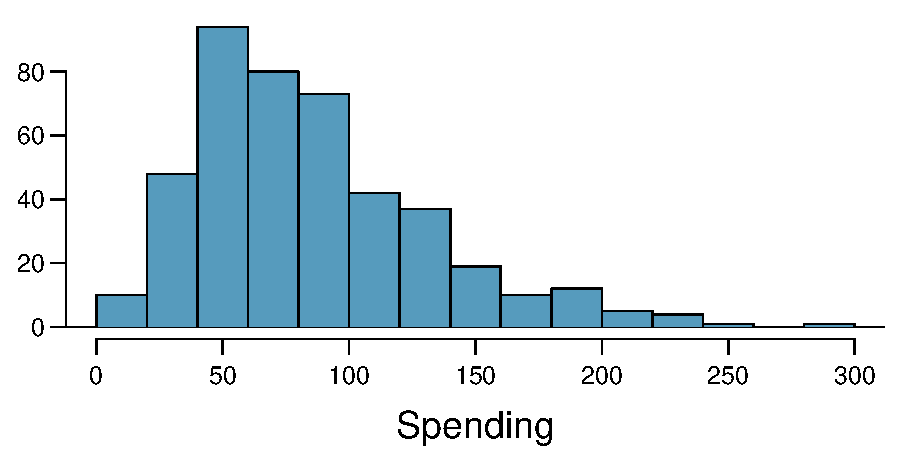
\includegraphics[width=100mm]{ch_inference_foundations_oi_biostat/figures/eoce/thanksgiving_spending_intro/thanksgiving_spending_intro_pop_hist.pdf}
	\end{center}
	\begin{parts}
		\item We are 95\% confident that the average spending of these 436 American 
		adults is between \$80.31 and \$89.11.
		\item This confidence interval is not valid since the distribution of spending 
		in the sample is right skewed.
		\item 95\% of random samples have a sample mean between \$80.31 and \$89.11.
		\item We are 95\% confident that the average spending of all American adults is 
		between \$80.31 and \$89.11.
		\item A 90\% confidence interval would be narrower than the 95\% confidence 
		interval.
		\item The margin of error is 4.4.
	\end{parts}
}{}

% 7 ODD (OI3, 4.13) edited

\eoce{\qt{Waiting at an ER, Part I\label{er_wait_intro}} A hospital administrator 
hoping to improve wait times decides to estimate the average emergency 
room waiting time at her hospital. She collects a simple random sample 
of 64 patients and determines the time (in minutes) between when they 
checked in to the ER until they were first seen by a doctor. A 95\% 
confidence interval based on this sample is (128 minutes, 147 minutes), 
which is based on the normal model for the mean. Determine whether the 
following statements are true or false, and explain your reasoning.
\begin{parts}
\item This confidence interval is not valid since we do not know if the 
population distribution of the ER wait times is nearly Normal.
\item We are 95\% confident that the average waiting time of these 64 emergency 
room patients is between 128 and 147 minutes.
\item We are 95\% confident that the average waiting time of all patients at 
this hospital's emergency room is between 128 and 147 minutes.
\item 95\% of random samples have a sample mean between 128 and 147 minutes.
\item A 99\% confidence interval would be narrower than the 95\% confidence 
interval since we need to be more sure of our estimate.
\item The margin of error is 9.5 and the sample mean is 137.5.
\item Halving the margin of error of a 95\% confidence interval requires doubling the sample size.
\end{parts}
}{}

\textD{\newpage}

% 8 EVEN (OI3, 4.16)

\eoce{\qt{Age at first marriage, Part I\label{age_at_first_marriage_intro}} 
The National Survey of Family Growth conducted by the Centers for Disease 
Control gathers information on family life, marriage and divorce, pregnancy, 
infertility, use of contraception, and men's and women's health. One of the 
variables collected on this survey is the age at first marriage. The histogram 
below shows the distribution of ages at first marriage of 5,534 randomly sampled 
women between 2006 and 2010. The average age at first marriage among these women 
is 23.44 with a standard deviation of 4.72.\footfullcite{data:nsfg:2010}
\begin{center}
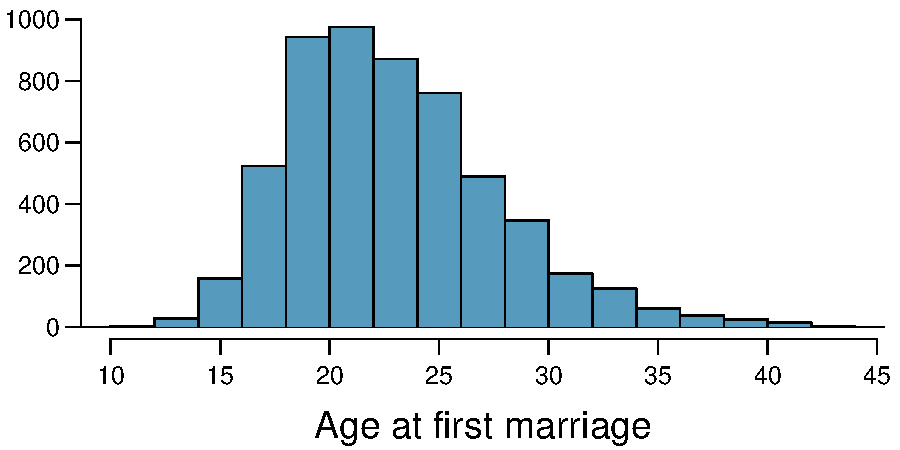
\includegraphics[width=0.65\textwidth]{ch_inference_foundations_oi_biostat/figures/eoce/age_at_first_marriage_intro/age_at_first_marriage_intro_hist.pdf}
\end{center}
Estimate the average age at first marriage of women using a 95\% confidence 
interval, and interpret this interval in context. Discuss any relevant 
assumptions.
}{}

% 9 oi_biostat section 5 spring 2020

\eoce{\qt{Mental health, Part II\label{gss_mental_health}} The General Social Survey (GSS) is a sociological survey used to collect data on demographic characteristics and attitudes of residents of the United States. The 2010 General Social Survey asked the question, "For how many days during the past 30 days was your mental health not good?" Based on responses from 1,151 US adults, the survey reported a 95\% confidence interval of (3.40, 4.24) days. Assume that the sampled US adults are representative of all US adults.
\begin{parts}
	\item Identify each of the following statements as true or false. Justify your answers.
	
	\begin{subparts}
		
		\item The confidence interval of (3.40, 4.24) contains the mean days out of the past 30 days that U.S. adults experienced poor mental health.
		
		\item There is a 95\% chance that the mean days out of the past 30 days that U.S. adults experienced poor mental health is within the confidence interval (3.40, 4.24).
		
		\item If we repeated this survey 1,000 times and constructed a 95\% confidence interval each time, then approximately 950 of those intervals would contain the true mean days out of the past 30 days that U.S. adults experienced poor mental health.
		
		\item The survey provides statistically significant evidence at the $\alpha = 0.05$ significance level that the mean days out of the past 30 days that U.S. adults experienced poor mental health is not 4.5 days.
		
		\item We can be 95\% confident that the mean days out of the past 30 days that U.S. adults experienced poor mental health is 3.82 days.
		
		\item We can be 95\% confident that the interval (3.40, 4.24) days contains the mean days out of the past 30 days that the sampled adults experienced poor mental health.
		
	\end{subparts}
	
	\item  Would you expect the 90\% confidence interval to be larger or smaller than the 95\% confidence interval? Explain your reasoning.
	
	\item  Calculate the 90\% confidence interval.

\end{parts}	
}{}

\textD{\newpage}

% 10 oi_biostat pset 4, spring 2020

\eoce{\qt{Leisure time, Part III\label{gss_leisure_time}} In 2010, the General Social Survey collected responses from 1,154 US residents. The survey is conducted face-to-face with an in-person interview of a randomly selected sample of adults. One of the questions on the survey is "After an average workday, about how many hours do you have to relax or pursue activities that you enjoy?" A 95\% confidence interval from the 2010 GSS survey for the collected answers is 3.53 to 3.83 hours. Identify each of the following statements as true or false. Explain your answers.
	
	\begin{parts}
		
		\item If the researchers wanted to report a confidence interval with a smaller margin of error based on the same sample of 1,154 Americans, the confidence interval would be larger.
		
		\item We can be 95\% confident that the interval (3.53, 3.83) hours contains the mean hours that the sampled adults have for leisure time after an average workday.
		
		\item The confidence interval of (3.53, 3.83) hours contains the mean hours that U.S. adults have for leisure time after an average workday.
		
		\item The survey provides statistically significant evidence at the $\alpha = 0.05$ significance level that the mean hours U.S. adults have for leisure time after the average workday is 3.6 hours.
		
		\item There is a 5\% chance that the interval (3.53, 3.83) hours does not contain the mean hours that U.S. adults have for leisure time after an average workday.
		
		\item The interval (3.53, 3.83) hours provides evidence at the $\alpha = 0.05$ significance level that U.S. adults, on average, have fewer than 3.9 hours of leisure time after a typical workday.
		
	\end{parts}

}{}\textD{\vspace{10mm}}


%_______________
\subsection{Hypothesis testing}

% 11 ODD (OI3, 4.17)

\eoce{\qt{Identify hypotheses, Part I\label{identify_hypotheses_1}} Write the null 
and alternative hypotheses in words and then symbols for each of the following 
situations.
\begin{parts}
\item New York is known as ``the city that never sleeps". A random sample of 25 
New Yorkers were asked how much sleep they get per night. Do these data provide 
convincing evidence that New Yorkers on average sleep less than 8 hours a night?
\item Employers at a firm are worried about the effect of March Madness, a 
basketball championship held each spring in the US, on employee productivity. 
They estimate that on a regular business day employees spend on average 15 
minutes of company time checking personal email, making personal phone calls, 
etc. They also collect data on how much company time employees spend on such non-
business activities during March Madness. They want to determine if these data 
provide convincing evidence that employee productivity decreases during March 
Madness.
\end{parts}
}{}

% 12 EVEN (OI3, 4.18)

\eoce{\qt{Identify hypotheses, Part II\label{identify_hypotheses_2}} 
Write the null and alternative hypotheses in words and using symbols 
for each of the following situations.
\begin{parts}
\item Since 2008, chain restaurants in California have been required to display 
calorie counts of each menu item. Prior to menus displaying calorie counts, the 
average calorie intake of diners at a restaurant was 1100 calories. After 
calorie counts started to be displayed on menus, a nutritionist collected data 
on the number of calories consumed at this restaurant from a random sample of 
diners. Do these data provide convincing evidence of a difference in the average 
calorie intake of a diners at this restaurant?
\item Based on the performance of those who took the GRE exam between July 1, 
2004 and June 30, 2007, the average Verbal Reasoning score was calculated to be 
462. In 2011 the average verbal score was slightly higher. Do these data provide 
convincing evidence that the average GRE Verbal Reasoning score has changed since 2004?
\end{parts}
}{}

\textD{\newpage}

% 13 ODD (OI3, 4.19)

\eoce{\qt{Online communication\label{online_communication}} A study suggests that the 
average college student spends 10 hours per week communicating with others 
online. You believe that this is an underestimate and decide to collect your 
own sample for a hypothesis test. You randomly sample 60 students from your 
dorm and find that on average they spent 13.5 hours a week communicating with 
others online. A friend of yours, who offers to help you with the hypothesis 
test, comes up with the following set of hypotheses. Indicate any errors you see.
\begin{align*}
H_0&: \bar{x} < 10~hours \\
H_A&: \bar{x} > 13.5~hours
\end{align*}
}{}

% 14 EVEN (OI3, 4.20)

\eoce{\qt{Age at first marriage, Part II\label{age_at_first_marriage_hyp_errors}} Exercise~\ref{age_at_first_marriage_intro} presents the results 
of a 2006 - 2010 survey showing that the average age of women at first marriage 
is 23.44. Suppose a social scientist believes that this value has increased in 
2012, but she would also be interested if she found a decrease. Below is how she 
set up her hypotheses. Indicate any errors you see.
\begin{align*}
H_0&: \bar{x} = 23.44~years \\
H_A&: \bar{x} > 23.44~years
\end{align*}
}{}

% 15 ODD (OI3, 4.21)

\eoce{\qt{Waiting at an ER, Part II\label{er_wait_ci_ht}} Exercise~\ref{er_wait_intro} 
provides a 95\% confidence interval for the mean waiting time at an emergency 
room (ER) of (128 minutes, 147 minutes). Answer the following questions based on
this interval.
\begin{parts}
\item A local newspaper claims that the average waiting time at this ER exceeds 
3 hours. Is this claim supported by the confidence interval? Explain your 
reasoning.
\item The Dean of Medicine at this hospital claims the average wait time is 2.2 
hours. Is this claim supported by the confidence interval? Explain your 
reasoning.
\item Without actually calculating the interval, determine if the claim of the 
Dean from part (b) would be supported based on a 99\% confidence interval?
\end{parts}
}{}


% 16 EVEN (OI3, 4.24)

\eoce{\qt{Gifted children, Part I\label{gifted_children_intro}} Researchers 
investigating characteristics of gifted children collected data from schools 
in a large city on a random sample of thirty-six children who were identified 
as gifted children soon after they reached the age of four. The following 
histogram shows the distribution of the ages (in months) at which these 
children first counted to 10 successfully. Also provided are some sample 
statistics.\footfullcite{Graybill:1994}

\begin{center}
\begin{minipage}[c]{0.6\textwidth}
\begin{center}
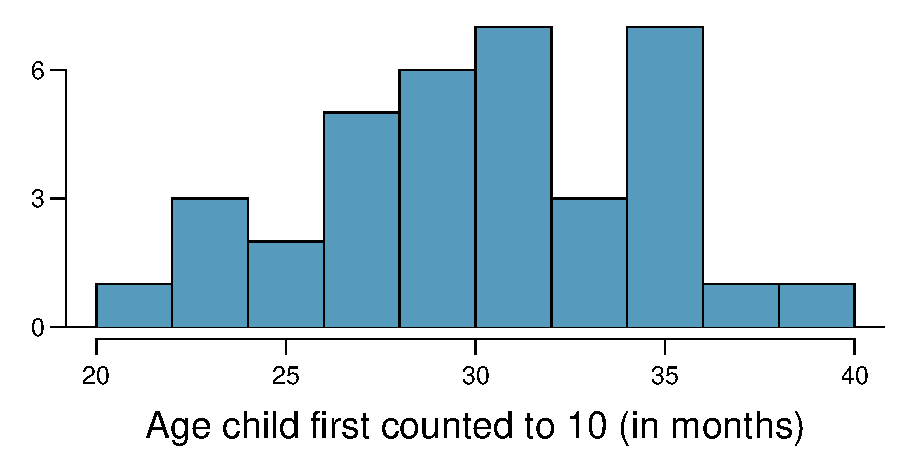
\includegraphics[width=\textwidth]{ch_inference_foundations_oi_biostat/figures/eoce/gifted_children_intro/gifted_children_ht_count_hist.pdf} 
\end{center}
\end{minipage}
\begin{minipage}[c]{0.1\textwidth}
\begin{tabular}{r | l}
n   & 36 \\
min & 21 \\
mean    & 30.69 \\
sd  & 4.31 \\
max & 39 
\end{tabular}
\end{minipage}
\end{center}

\begin{parts}
\item Are conditions for inference satisfied?
\item Suppose an online survey reports that children first count to 10 successfully when 
they are 32 months old, on average. Perform a hypothesis test to evaluate if 
these data provide convincing evidence that the average age at which gifted 
children first count to 10 successfully is less than the general average of 32 
months. Use a significance level of 0.10.
\item Interpret the p-value in context of the hypothesis test and the data. 
\item Calculate a 90\% confidence interval for the average age at which gifted children first count to 10 successfully.
\item Do your results from the hypothesis test and the confidence interval agree? Explain.
\end{parts}
}{}

\textD{\newpage}

% 17 ODD (OI3, 4.23)

\eoce{\qt{Nutrition labels\label{nutrition_labels}} The nutrition label on a bag of 
	potato chips says that a one ounce (28~gram) serving of potato chips has 130 
	calories and contains ten grams of fat, with three grams of saturated fat. A 
	random sample of 35 bags yielded a sample mean of 134 calories with a standard 
	deviation of 17 calories. Is there evidence that the nutrition label does not 
	provide an accurate measure of calories in the bags of potato chips? We have 
	verified the independence, sample size, and skew conditions are satisfied.
}{}


% 18 EVEN (OI3, 4.25) edited

\eoce{\qt{Waiting at an ER, Part III\label{er_wait_ht}} The hospital administrator 
mentioned in Exercise~\ref{er_wait_intro} randomly selected 64 patients and 
measured the time (in minutes) between when they checked in to the ER and the 
time they were first seen by a doctor. The average time is 137.5 minutes and 
the standard deviation is 39 minutes. She is getting grief from her supervisor 
on the basis that the wait times in the ER has increased greatly from last 
year's average of 127 minutes. However, she claims that the increase is 
probably just due to chance. 
\begin{parts}
\item Calculate a 95\% confidence interval. Is the change in wait times statistically significant at the $\alpha = 0.05$ level?
\item Would the conclusion in part (a) change if the significance 
level were changed to $\alpha = 0.01$?
\item Is the supervisor justified in criticizing the hospital administrator regarding the change in ER wait times? How might you present an argument in favor of the administrator?
\end{parts}
}{}

% 19 oi_biostat, pset_04, spring 2016

\eoce{\qt{Birth weights\label{birth_weights}} Suppose an investigator takes a random sample of $n = 50$ birth weights from several teaching hospitals located in an inner-city neighborhood. In her random sample, the sample mean $\overline{x}$ is 3,150 grams and the standard deviation is 250 grams.
	\begin{parts}
		\item Calculate a 95\% confidence interval for the population mean birth weight in these hospitals.
		\item The typical weight of a baby at birth for the US population is 3,250 grams. The investigator suspects that the birth weights of babies in these teaching hospitals is different than 3,250 grams, but she is not sure if it is smaller (from malnutrition) or larger (because of obesity prevalence in mothers giving birth at these hospitals). Carry out the hypothesis test that she would conduct.
	\end{parts}	
}{}

% 20 EVEN (OI3, 4.26)

\eoce{\qt{Gifted children, Part II\label{gifted_children_ht}} Exercise~\ref{gifted_children_intro} describes a study on gifted 
children. In this study, along with variables on the children, the researchers 
also collected data on the mother's and father's IQ of the 36 randomly sampled 
gifted children. The histogram below shows the distribution of mother's IQ.  
Also provided are some sample statistics.

\begin{center}
\begin{minipage}[c]{0.6\textwidth}
\begin{center}
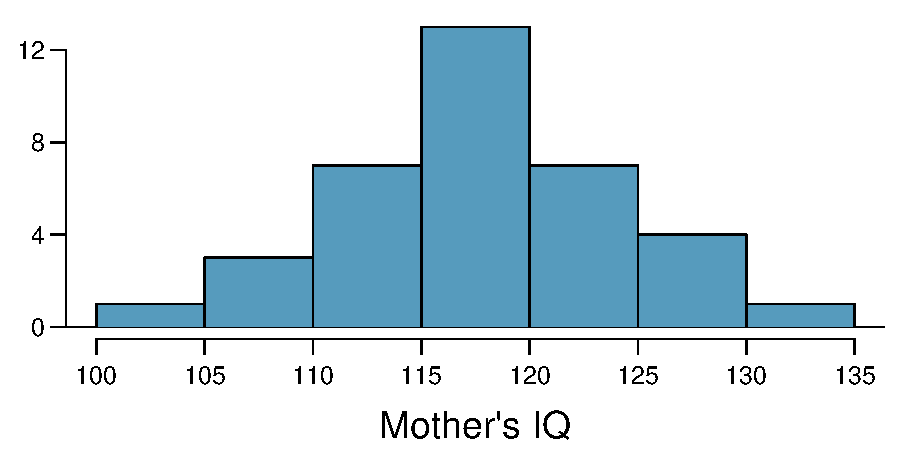
\includegraphics[width=\textwidth]{ch_inference_foundations_oi_biostat/figures/eoce/gifted_children_ht/gifted_children_ht_momIQ_hist.pdf} 
\end{center}
\end{minipage}
\begin{minipage}[c]{0.1\textwidth}
\begin{tabular}{r | l}
n   & 36 \\
min & 101 \\
mean    & 118.2 \\
sd  & 6.5 \\
max & 131 
\end{tabular}
\end{minipage}
\end{center}

\begin{parts}
\item Perform a hypothesis test to evaluate if these data provide convincing 
evidence that the average IQ of mothers of gifted children is different than the 
average IQ for the population at large, which is 100. Use a significance level 
of 0.10.
\item Calculate a 90\% confidence interval for the average IQ of mothers of 
gifted children.
\item Do your results from the hypothesis test and the confidence interval 
agree? Explain.
\end{parts}
}{}

\textD{\newpage}

% 21 ODD (OI3, 4.29)

\eoce{\qt{Testing for fibromyalgia\label{errors_fibromyalgia}} A patient named Diana 
was diagnosed with fibromyalgia, a long-term syndrome of body pain, and was 
prescribed anti-depressants. Being the skeptic that she is, Diana didn't 
initially believe that anti-depressants would help her symptoms. However after 
a couple months of being on the medication she decides that the 
anti-depressants are working, because she feels like her symptoms are in fact 
getting better.
\begin{parts}
\item Write the hypotheses in words for Diana's skeptical position when she 
started taking the anti-depressants.
\item What is a Type~1 Error in this context?
\item What is a Type~2 Error in this context?
\end{parts}
}{}


% 22 EVEN (OI3, 4.30)

\eoce{\qt{Testing for food safety\label{errors_food_safety}} A food safety inspector 
is called upon to investigate a restaurant with a few customer reports of poor 
sanitation practices. The food safety inspector uses a hypothesis testing 
framework to evaluate whether regulations are not being met. If he decides 
the restaurant is in gross violation, its license to serve food will be revoked.
\begin{parts}
\item Write the hypotheses in words.
\item What is a Type~1 Error in this context?
\item What is a Type~2 Error in this context?
\item Which error is more problematic for the restaurant owner? Why?
\item Which error is more problematic for the diners? Why?
\item As a diner, would you prefer that the food safety inspector requires 
strong evidence or very strong evidence of health concerns before revoking a 
restaurant's license? Explain your reasoning.
\end{parts}
}{}

% 23 ODD (OI3, 4.31)

\eoce{\qtq{Which is higher\label{which_higher_found_inf}} In each part below, there is a value of interest and two 
scenarios (I and II). For each part, report if the value of interest is larger 
under scenario I, scenario II, or whether the value is equal under the scenarios.
\begin{parts}
\item The standard error of $\bar{x}$ when $s = 120$ and 
(I) n = 25 or (II) n = 125.
\item The margin of error of a confidence interval when the confidence level is 
(I) 90\% or (II) 80\%.
\item The p-value for a Z-statistic of 2.5 when (I) n = 500 or (II) n = 1000.
\item The probability of making a Type~2 Error when the alternative hypothesis 
is true and the significance level is (I) 0.05 or (II) 0.10.
\end{parts}
}{}

% 24 EVEN (OI3, 4.32)

\eoce{\qt{True or false\label{tf_found_inf}} Determine if the following statements are true or false, and 
explain your reasoning. If false, state how it could be corrected.
\begin{parts}
\item If a given value (for example, the null hypothesized value of a parameter) 
is within a 95\% confidence interval, it will also be within a 99\% confidence 
interval.
\item Decreasing the significance level ($\alpha$) will increase the probability 
of making a Type~1 Error.
\item Suppose the null hypothesis is $\mu = 5$ and we fail to reject $H_0$. 
Under this scenario, the true population mean is 5.
\item If the alternative hypothesis is true, then the probability of making a 
Type~2 Error and the power of a test add up to 1.
\item With large sample sizes, even small differences between the null value and 
the true value of the parameter, a difference often called the effect size
\index{effect size}, will be identified as statistically significant.
\end{parts}
}{}
